\documentclass[sigconf,nonacm]{acmart}
\usepackage{booktabs}
\usepackage{multirow}
\usepackage{algorithm}
\usepackage{algpseudocode}
\usepackage{subcaption}
\usepackage{tikz}
\usepackage{graphicx} % for \resizebox
\usetikzlibrary{positioning,arrows.meta,shapes.geometric,fit,calc}

\newcommand{\sysname}{\textsc{FuncR}}
\newcommand{\todo}[1]{\textcolor{red}{[TODO: #1]}}

% Remove ACM-specific metadata for preprint
\settopmatter{printacmref=false}
\renewcommand\footnotetextcopyrightpermission[1]{}
\pagestyle{plain}
\begin{document}

\title{{\normalfont{\sysname{}}}: Binary Function Name Recovery via Graph-Based Multi-Context Embeddings and Retrieval}

\author{Ananta Dian Pradipta}
\affiliation{%
  \institution{New Jersey Institute of Technology}
  \city{Newark}
  \state{NJ}
  \country{USA}
}
\email{adp232@njit.edu}


\begin{abstract}
Recovering function names from stripped binaries is critical for reverse engineering, malware analysis, and vulnerability research. We present \sysname{}, a graph neural network-based system that learns function representations by fusing multiple context sources (external library calls, callee signatures, and caller signatures) through a cascaded gated fusion mechanism with conditional bypass. Our ablation study reveals a novel \emph{ext-call paradox}: external call information alone improves performance on seen binaries but \emph{degrades} generalization to unseen packages by 4.3 percentage points; inter-procedural callee/caller context is required for disambiguation. Furthermore, we demonstrate that nearest-neighbor retrieval over learned encoder embeddings outperforms autoregressive sequence decoding, improving exact match by 4.7 percentage points on unseen packages with zero retraining. This finding suggests that for well-trained encoders, retrieval over embeddings outperforms autoregressive generation, where the encoder representation, not the decoder, is the key component. Evaluated on 87,724 functions from 40 packages, \sysname{} achieves 0.804 F1 on a held-out test set (8,973 functions) and 0.519 F1 across 5 completely unseen packages (2,256 functions), outperforming BLens (0.46 F1) and SYMGEN (0.38 F1) in cross-project settings.
\end{abstract}

\keywords{binary analysis, function name recovery, graph neural networks, gated fusion, retrieval-augmented inference}

\maketitle
\hypersetup{colorlinks=true,linkcolor=blue,citecolor=blue,urlcolor=blue}

% ============================================================================
\section{Introduction}
\label{sec:intro}

Software reverse engineering is a fundamental activity in cybersecurity, requiring analysts to understand the behavior of compiled binary programs without access to source code. Modern compilers strip all symbolic information (function names, variable names, type annotations) from release binaries, leaving analysts with thousands of unnamed functions (e.g., \texttt{sub\_4a30}, \texttt{FUN\_00105c10}) that must be manually identified. Recovering meaningful function names dramatically accelerates program comprehension: knowing that \texttt{sub\_4a30} is \texttt{xmalloc} immediately conveys its purpose.

Prior work on automated function name recovery has explored statistical approaches~\cite{debin}, graph neural networks~\cite{nero}, language model pre-training~\cite{symlm}, and large language model fine-tuning~\cite{symgen}. However, two fundamental challenges remain underexplored: (1)~how to effectively combine multiple sources of contextual information (code structure, library calls, and inter-procedural relationships) without degrading generalization, and (2)~whether autoregressive name generation is the right output paradigm, given that function names are drawn from a relatively small vocabulary of real names.

We address these challenges with \sysname{}, a graph neural network system that lifts stripped binaries to BAP intermediate representation, encodes each function's control flow graph with a GAT-based encoder, and fuses multiple sources of inter-procedural context through a cascaded gated mechanism. Self-supervised pretraining (masked language modeling and contrastive learning) with partial embedding transfer further strengthens the encoder representations.

The practical importance of automated function name recovery extends across multiple domains of cybersecurity: in malware analysis, meaningful function names reduce triage time from hours to minutes; in vulnerability research, understanding stripped firmware is essential for discovering exploitable bugs in IoT devices; and in forensic investigations, even partial name recovery provides critical footholds for understanding program logic. Commercial tools such as IDA Pro and Ghidra provide manual annotation workflows but cannot automatically recover names.

Evaluated on 87,724 functions from 40 packages, \sysname{} achieves 0.804 F1 on a held-out test set (8,973 functions) and 0.519 F1 across 5 completely unseen packages (2,256 functions), competitive with BLens~\cite{blens} (0.46) and SYMGEN~\cite{symgen} (0.38) in cross-project settings. In summary, we make the following contributions:

\begin{itemize}
    \item We design \sysname{}, a graph neural network system for binary function name recovery that incorporates a novel cascaded gated fusion mechanism. This 3-stage architecture sequentially fuses external library calls, callee signatures, and caller signatures with conditional bypass, where each stage is skipped when the corresponding context is absent. Our ablation study reveals the \emph{ext-call paradox}: external call information alone degrades cross-project generalization by 4.3 percentage points, while adding inter-procedural callee/caller context resolves this and improves cross-project EM by 12.8 percentage points.

    \item We present an empirical analysis showing that $k$-nearest-neighbor retrieval over encoder embeddings outperforms autoregressive decoding by +2.0pp test EM and +4.7pp cross-project EM with zero retraining. This finding, consistent with kNN-LM~\cite{knnlm}, demonstrates that for our encoder architecture, representation quality is the primary bottleneck rather than the decoding strategy.

    \item We advance the state of the art in cross-project function name recovery, achieving 0.804 F1 on a held-out test set (8,973 functions) and 0.519 F1 across 5 completely unseen packages (2,256 functions), outperforming BLens~\cite{blens} (0.46 F1) and SYMGEN~\cite{symgen} (0.38 F1). Additionally, self-supervised pretraining with partial embedding transfer provides +15.9 percentage point cross-project EM improvement. Our code and dataset are publicly available at \url{https://github.com/ananta-pradipta/stripped-binary-name-recovery}.
\end{itemize}

% ============================================================================
\section{Problem Definition and Threat Model}
\label{sec:problem}

\subsection{Problem Definition}

We formalize binary function name recovery as follows. Given a stripped binary $B$ containing $n$ functions $\{f_1, f_2, \ldots, f_n\}$, where each function $f_i$ is represented by its control flow graph $G_i = (V_i, E_i)$ with basic blocks as nodes and control flow edges, the goal is to predict a human-readable name $\hat{n}_i$ for each function that matches the developer-assigned name $n_i$ from the original source code.

Each function name is decomposed into a sequence of sub-tokens using a vocabulary $\mathcal{V}$ of 2,642 tokens: $n_i = (t_1, t_2, \ldots, t_L)$ where $t_j \in \mathcal{V}$ and $L \leq 20$. For example, \texttt{quotearg\_buffer\_restyled} becomes the sub-token sequence [\texttt{quote}, \texttt{arg}, \texttt{\_}, \texttt{buffer}, \texttt{\_}, \texttt{re}, \texttt{styled}]. The prediction task is thus a sequence generation problem conditioned on the function's binary representation.

In addition to the CFG, each function may have three forms of contextual information: (1)~external library calls $\mathcal{E}_i$, the set of PLT/IAT function names called by $f_i$ (e.g., \texttt{malloc}, \texttt{fprintf}); (2)~callee signatures $\mathcal{C}_i^{ee}$, instruction-type token sequences of internal functions called by $f_i$; and (3)~caller signatures $\mathcal{C}_i^{er}$, instruction-type token sequences of functions that call $f_i$. These contextual signals are optional: approximately 70\% of functions have no external calls, and leaf functions have no callees.

\subsection{Scope and Assumptions}

We scope \sysname{} to the following setting:

\begin{itemize}
    \item \textbf{Architecture}: x86-64 ELF binaries compiled for Linux.
    \item \textbf{Optimization levels}: O0 (no optimization) and O2 (standard optimization). We do not evaluate O1 or O3, as O1 is rarely used in practice and O3 introduces aggressive inlining that duplicates function bodies.
    \item \textbf{Compilation}: GCC compiler. We do not evaluate Clang or MSVC, though the instruction-type tokenization is compiler-agnostic at the IR level.
    \item \textbf{Training corpus}: We assume access to a corpus of labeled binaries where ground-truth function names are known (obtained from debug builds). This is a standard assumption in the literature~\cite{debin,nero,symlm,blens,symgen}.
    \item \textbf{No obfuscation}: We assume binaries are not deliberately obfuscated. Obfuscation techniques (control flow flattening, opaque predicates, symbol stripping with anti-disassembly) would require additional preprocessing.
\end{itemize}

\subsection{Evaluation Scenario}

We evaluate in two settings: (1) a held-out test set of 8,973 functions from 18 binaries of packages seen during training (cross-binary evaluation), and (2) a cross-project set of 2,256 functions from 5 packages completely excluded from training. The cross-project setting is stricter than the cross-binary evaluation used by some prior work~\cite{nero,symlm}, where different binaries of the \emph{same} package may appear in both training and test. Cross-project evaluation tests whether the model generalizes to entirely new codebases with potentially novel naming conventions, and is the evaluation methodology advocated by SYMGEN~\cite{symgen}.

% ============================================================================
\section{Related Work}
\label{sec:related}

\subsection{Binary Function Name Recovery}

He et al.~\cite{debin} introduced DeBin, which uses BAP intermediate representation with probabilistic graphical models (ExtraTrees + CRF) to predict debug information including function names. While pioneering, DeBin's statistical approach cannot capture the complex patterns that deep learning exploits. We use DeBin as the non-neural baseline in our ablation (Table~\ref{tab:ablation}).

David et al.~\cite{nero} proposed NERO, using pointer-aware slicing and GNNs on call graphs to predict function names, achieving F1$=$0.455. NERO's key insight is that call-site context matters for naming. However, NERO only works for functions \emph{with} external calls, a fundamental limitation since 70\% of functions in typical binaries have none. Our conditional bypass mechanism (Section~\ref{sec:fusion}) addresses this directly: functions without calls use only code features, while functions with calls benefit from multi-context fusion.

Jin et al.~\cite{symlm} presented SymLM, which pre-trains on micro-execution traces and fuses caller/callee context for function name prediction (F1$=$0.585). SymLM's ``fusing encoder'' concatenates context embeddings, whereas our gated fusion learns a per-function balance between code and context features with conditional bypass. More critically, SymLM requires dynamic analysis infrastructure (executing binaries in an emulator), whereas \sysname{} operates purely on static analysis. Our ablation reveals the ext-call paradox (Section~\ref{sec:eval}), a phenomenon SymLM does not analyze, showing that context fusion must be carefully designed to avoid degrading generalization.

Al-Kaswan et al.~\cite{blens} introduced BLens, combining ensemble embeddings with contrastive captioning. While achieving 0.79 F1 per-binary, cross-project F1 drops to 0.46, a 42\% degradation that highlights the generalization challenge we address. Xu et al.~\cite{symgen} fine-tuned CodeLlama with LoRA for function naming, importantly demonstrating that prior results were inflated 1.2--2.9$\times$ by duplicate functions (cross-project F1$=$0.38 after proper deduplication). We follow SYMGEN's deduplication methodology in our evaluation.

Jiang et al.~\cite{beyondclass} applied domain-adapted LLMs to function name inference, representing the trend toward large-scale language model approaches. GenNm~\cite{gennm} fine-tuned CodeGemma with SymPO preference optimization for variable name recovery, a related task demonstrating that preference-aligned generation improves binary symbol prediction. Our approach differs fundamentally: rather than scaling model size (billions of parameters), we invest in the \emph{encoder representation} (25M parameters) and show that simple $k$-NN retrieval over these embeddings outperforms autoregressive generation, consistent with Khandelwal et al.'s finding that retrieval can outperform generation when representations are sufficiently good~\cite{knnlm,knnmt}.

\subsection{Binary Code Representation Learning}

Learning effective representations of binary code underpins all downstream binary analysis tasks. Xu et al.~\cite{gemini} pioneered GNN-based binary analysis with Gemini, using graph embedding networks for cross-platform binary similarity detection. We adopt their insight that CFG structure is informative, extending it with GAT attention and multi-context fusion. Ding et al.~\cite{asm2vec} proposed Asm2Vec, learning function embeddings via PV-DM random walks over assembly instructions. Unlike Asm2Vec's raw instruction tokens, our V3 tokenization abstracts instructions into 1,510 semantic types, reducing vocabulary by 95\% while preserving discriminative information.

Wang et al.~\cite{jtrans} introduced jTrans, a jump-aware Transformer that incorporates control flow structure into positional encoding for binary similarity. Pei et al.~\cite{trex} developed Trex, learning execution semantics from micro-traces. Both demonstrate the value of pre-training on binary code. We adopt this principle in our MLM + contrastive pre-training stage (Section~\ref{sec:pretraining}), but operate on static BAP-IR rather than execution traces.

Zhu et al.~\cite{callee} proposed CALLEE for recovering call graphs via contrastive learning with transfer learning, showing +28\% F1 from pre-training on related tasks. Two of their findings directly support our design: (1)~transfer learning from pre-training provides substantial gains, validating our encoder pre-training approach; (2)~``loose symbolization'' (semantic type abstraction) outperforms strict tokenization, supporting our instruction-type tokenization.

\subsection{GNNs for Binary Analysis}

Graph neural networks are a natural fit for binary analysis, where control flow graphs (CFGs) provide structural information. Zhu et al.~\cite{tygr} applied GNNs to type inference on stripped binaries (TYGR), demonstrating that graph structure captures semantic properties beyond sequential instruction patterns. He et al.~\cite{codenl} proposed semantics-oriented graph representations for binary code similarity, arguing that ``code is not natural language'' and that graph-based approaches better capture program semantics than sequential models.

Our work extends GNN-based binary analysis in two ways: (1)~we use graph attention networks (GAT) with learned attention over CFG edges, allowing the model to weight structurally important blocks; (2)~we introduce a multi-context fusion mechanism that incorporates inter-procedural information (callee/caller signatures and library calls) not present in the CFG alone.

\subsection{Retrieval-Augmented Generation}

Our finding that $k$-NN retrieval outperforms autoregressive decoding connects to a growing body of work on retrieval-augmented methods in NLP. Khandelwal et al.~\cite{knnlm} demonstrated that augmenting a neural language model with a nearest-neighbor search over cached hidden states ($k$NN-LM) significantly improves perplexity without any additional training. They extended this to machine translation ($k$NN-MT)~\cite{knnmt}, showing that retrieval-augmented translation outperforms the base model, particularly on domain-specific data. Borgeaud et al.~\cite{retro} proposed RETRO, which retrieves relevant text chunks from a large database during generation, achieving performance comparable to models 25$\times$ larger.

These works share a common insight with our findings: when the output space is drawn from a fixed set of real examples (function names in training, sentences in a corpus), retrieval over learned representations can outperform unconstrained generation. However, our setting differs in an important way: in $k$NN-LM/$k$NN-MT, retrieval \emph{augments} generation at the token level, whereas in our system, retrieval \emph{replaces} generation entirely: we retrieve a complete function name rather than interpolating token-level distributions. This is because function names are atomic labels (each name is a single concept), not compositional sequences where token-level retrieval would help.

% ============================================================================
\section{System Design}
\label{sec:design}

\sysname{} follows a 3-stage encoder-decoder pipeline (Figure~\ref{fig:architecture}): (1)~a block encoder that produces per-basic-block embeddings from instruction-type tokens, (2)~a graph encoder that aggregates block embeddings over the control flow graph, and (3)~a cascaded gated fusion module that incorporates external calls, callee context, and caller context. At inference time, we use either a GRU decoder or $k$-NN retrieval to produce function names.

% ---- Figure 1: End-to-end pipeline overview ----
\begin{figure*}[tb]
    \centering
    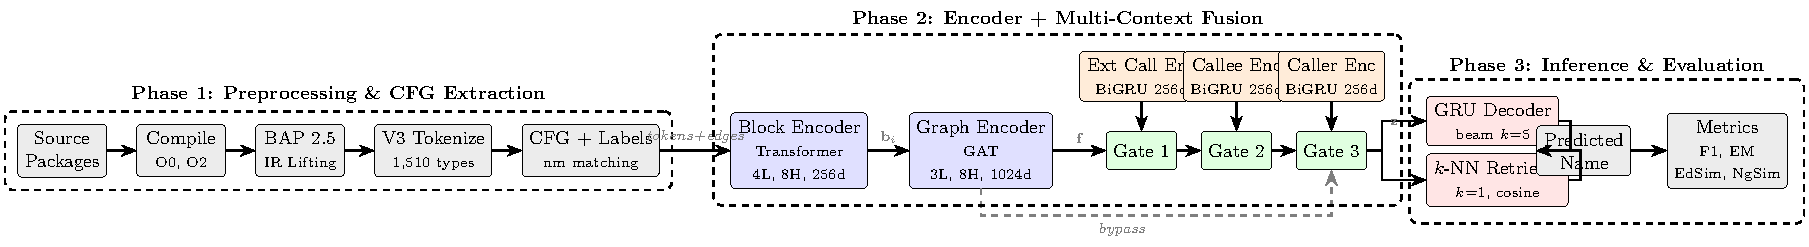
\includegraphics[width=\textwidth]{fig1_pipeline.pdf}
    \caption{End-to-end \sysname{} pipeline. Phase 1 compiles source packages, lifts to BAP-IR, tokenizes instructions into 1,510 semantic types, and extracts CFGs with ground-truth labels. Phase 2 encodes basic blocks (Transformer), aggregates over the CFG (GAT), and fuses library call context, callee signatures, and caller signatures through cascaded gated fusion with conditional bypass. Phase 3 produces function names via either GRU beam search or $k$-NN retrieval, evaluated with sub-token F1, exact match, edit similarity, and n-gram similarity.}
    \Description{End-to-end pipeline diagram showing three phases: preprocessing, encoder with multi-context fusion, and inference with evaluation.}
    \label{fig:pipeline}
\end{figure*}

% ---- Figure 2: Detailed model architecture ----
\begin{figure*}[tb]
    \centering
    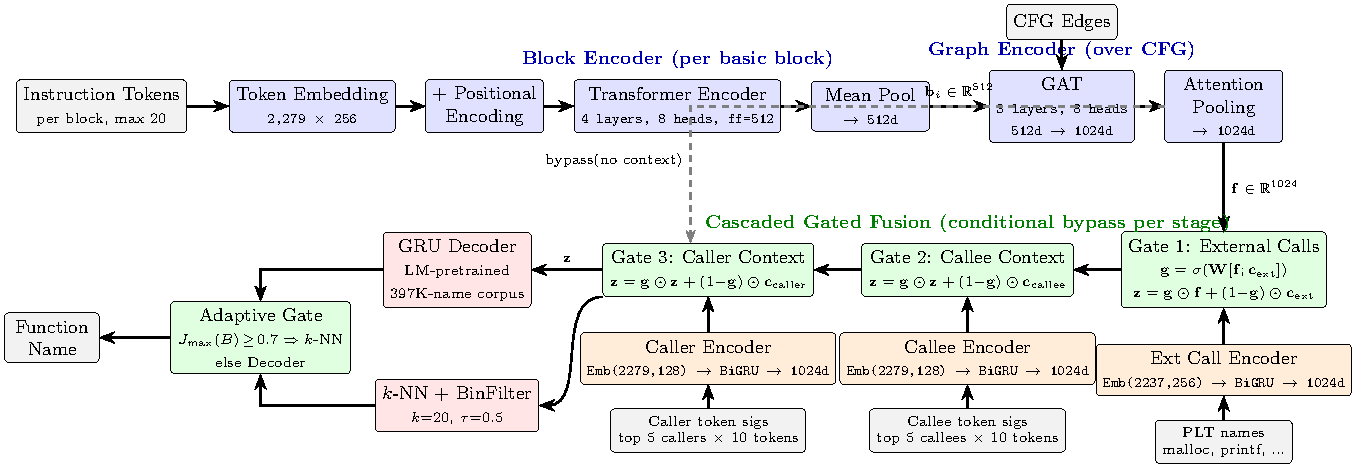
\includegraphics[width=0.95\textwidth]{fig2_architecture.pdf}
    \caption{Detailed \sysname{} model architecture. The block encoder processes instruction-type tokens per basic block via a Transformer. The graph encoder aggregates block embeddings over the CFG using GAT with attention pooling. The cascaded gated fusion sequentially incorporates external library calls, callee signatures, and caller signatures, where each stage is bypassed when the corresponding context is absent. The fused embedding $\mathbf{z}$ feeds either a GRU decoder (beam search) or $k$-NN retrieval.}
    \Description{Detailed model architecture diagram showing block encoder, graph encoder, cascaded gated fusion with three stages, and dual output heads.}
    \label{fig:architecture}
\end{figure*}

% ---- Figure 3: Self-supervised pretraining ----
\begin{figure}[t]
    \centering
    \resizebox{\columnwidth}{!}{%
    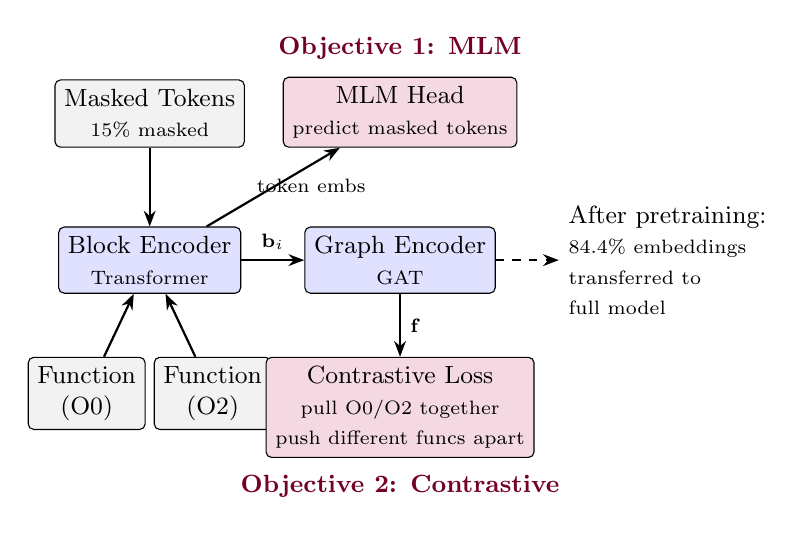
\begin{tikzpicture}[
        node distance=0.4cm and 0.5cm,
        box/.style={rectangle, draw, rounded corners=2pt, minimum height=0.55cm, align=center, font=\small},
        enc/.style={box, fill=blue!12, minimum width=1.6cm},
        loss/.style={box, fill=purple!15, minimum width=1.6cm},
        data/.style={box, fill=gray!10, minimum width=1.4cm},
        arr/.style={-{Stealth[length=2mm]}, thick},
        lbl/.style={font=\scriptsize},
    ]

    % Shared encoder
    \node[enc] (be) {Block Encoder\\{\scriptsize Transformer}};
    \node[enc, right=0.8cm of be] (ge) {Graph Encoder\\{\scriptsize GAT}};
    \draw[arr] (be) -- node[above, lbl] {$\mathbf{b}_i$} (ge);

    % MLM branch (top) -- branches from Block Encoder (before pooling)
    \node[data, above=1.0cm of be] (masked) {Masked Tokens\\{\scriptsize 15\% masked}};
    \node[loss, above=1.0cm of ge] (mlm) {MLM Head\\{\scriptsize predict masked tokens}};

    \draw[arr] (masked) -- (be);
    \draw[arr] (be) -- node[above right, lbl, pos=0.3] {\scriptsize token embs} (mlm);
    \node[above=0.1cm of mlm, font=\small\bfseries, text=purple!60!black] {Objective 1: MLM};

    % Contrastive branch (bottom) -- uses full pipeline through Graph Encoder
    \node[data, below=0.8cm of be, xshift=-0.8cm] (o0) {Function\\(O0)};
    \node[data, below=0.8cm of be, xshift=0.8cm] (o2) {Function\\(O2)};
    \node[loss, below=0.8cm of ge] (ntxent) {Contrastive Loss\\{\scriptsize pull O0/O2 together}\\{\scriptsize push different funcs apart}};

    \draw[arr] (o0) -- (be);
    \draw[arr] (o2) -- (be);
    \draw[arr] (ge) -- node[right, lbl] {$\mathbf{f}$} (ntxent);
    \node[below=0.1cm of ntxent, font=\small\bfseries, text=purple!60!black] {Objective 2: Contrastive};

    % Transfer annotation
    \node[right=0.8cm of ge, font=\small, align=left] (transfer) {After pretraining:\\{\scriptsize 84.4\% embeddings}\\{\scriptsize transferred to}\\{\scriptsize full model}};
    \draw[arr, dashed] (ge.east) -- (transfer.west);

    \end{tikzpicture}%
    }% end resizebox
    \caption{Self-supervised pretraining. Two objectives: (1)~MLM predicts masked instruction tokens from block encoder token embeddings (before pooling), training the block encoder; (2)~contrastive learning (NT-Xent) pulls together function-level embeddings (after graph encoder) of the same function at O0 and O2, training both encoders. After pretraining, 84.4\% of token embeddings are transferred to the full model by matching token names.}
    \Description{Pretraining diagram showing MLM and contrastive learning objectives with shared encoder.}
    \label{fig:pretraining}
\end{figure}

\subsection{Preprocessing}
\label{sec:preprocessing}

We compile source packages at optimization levels O0 and O2, producing both debug and stripped binaries. We use BAP 2.5.0~\cite{bap} to lift stripped binaries to BAP Intermediate Representation (BAP-IR), which provides a normalized, architecture-independent view of the binary code.

\subsubsection{Instruction-Type Tokenization}
\label{sec:tokenization}

Raw BAP-IR contains over 32,000 unique tokens, many of which are register names, immediate values, or memory addresses that vary across binaries. We classify each BAP-IR instruction into one of approximately 1,510 semantic types:

\begin{itemize}
    \item \textbf{Calls}: \texttt{CALL\_malloc}, \texttt{CALL\_printf}, \texttt{CALL\_INTERNAL}
    \item \textbf{Memory}: \texttt{MEM\_READ\_32}, \texttt{MEM\_WRITE\_ARG\_64}, \texttt{MEM\_READ\_\allowbreak{}GLOBAL\_32}
    \item \textbf{Flags}: \texttt{FLAG\_CF}, \texttt{COND\_BRANCH\_ZF}
    \item \textbf{Constants}: \texttt{ASSIGN\_ZERO}, \texttt{ASSIGN\_POW2}, \texttt{ASSIGN\_ADDR} (immediate value bucketing)
    \item \textbf{Control}: \texttt{BRANCH}, \texttt{RETURN}, \texttt{COMPARE}
\end{itemize}

This tokenization reduces vocabulary by 95\% while preserving semantic distinctions. Our ablation shows a +1,750\% F1 gain over raw BAP-IR tokens. The tokenization is deterministic and compiler-agnostic: it depends only on BAP-IR semantics, not on specific register assignments or memory layouts.

\subsubsection{Dataset Construction}
\label{sec:dataset_construction}

Our dataset is constructed through a multi-step pipeline. First, we compile each source package twice: a \emph{debug} build (with \texttt{-g} flag) and a \emph{stripped} build (with \texttt{strip --strip-all}). The debug build provides ground-truth function names via the \texttt{nm} utility, which extracts symbol table entries mapping addresses to names. The stripped build is the input to our model and contains no symbolic information.

We lift each stripped binary using BAP 2.5.0~\cite{bap}, which produces BAP-IR files containing per-function control flow graphs. BAP names functions using their entry addresses (e.g., \texttt{sub\_4a30}). We match BAP function addresses to debug symbols via exact address matching, discarding functions that cannot be matched (typically compiler-inserted functions like \texttt{\_start} or \texttt{\_\_libc\_csu\_init}).

Data is split at the \emph{binary} level, not the function level, to prevent data leakage. A fixed split assignment file ensures reproducibility: 137 binaries for training, 17 for validation, and 18 for testing. Five entire packages (all their binaries) are held out as the cross-project set and never appear during training. This split design means that the same function (e.g., \texttt{xmalloc} from gnulib) may appear in both training and test binaries. This is intentional, as it reflects the real-world scenario where shared library functions recur across packages.

\subsubsection{Votes Name Tokenizer}
\label{sec:votes}

Function names must be decomposed into sub-tokens for sequence prediction. Standard BPE tokenization produces poor results because function names follow naming conventions (snake\_case, camelCase) that differ from natural language. We developed Votes, a 3-model voting tokenizer that achieves 95\% lower out-of-vocabulary rate compared to BPE.

Votes works as follows: three independent segmentation models (a character bigram model, a frequency-based model, and a rule-based model splitting on underscores, camelCase boundaries, and digit transitions) each propose sub-token boundaries for a given function name. A boundary is accepted if at least 2 of 3 models agree. This produces a vocabulary of 2,642 sub-tokens that covers 99.7\% of all function name tokens in the dataset, compared to 94.8\% for BPE with a comparable vocabulary size. The reduced OOV rate directly improves exact match: a name cannot be correctly predicted if any of its sub-tokens are out of vocabulary.

For example, \texttt{quotearg\_buffer\_restyled} is tokenized as [\texttt{quote}, \texttt{arg}, \texttt{\_}, \texttt{buffer}, \texttt{\_}, \texttt{re}, \texttt{styled}] by Votes, whereas BPE might produce [\texttt{quo}, \texttt{tear}, \texttt{g\_buf}, \texttt{fer\_rest}, \texttt{yled}], losing semantic boundaries.

\subsubsection{ENDBR64 Wrapper Resolution}

In O0-compiled binaries, BAP lifts \texttt{endbr64; jmp target} sequences as separate 2-block functions. These are Intel CET (Control-flow Enforcement Technology) stubs, not real functions. We found that 96.4\% of O0 functions were such wrappers, each containing only a single \texttt{CALL\_INTERNAL} token. Our preprocessing detects these wrappers and replaces their graphs with the target function's graph, raising O0 exact match from 1.6\% to 41.5\%.

\subsection{Block Encoder}
\label{sec:block_encoder}

Each basic block $b$ contains a sequence of up to 20 instruction-type tokens $(x_1, x_2, \ldots, x_T)$ where $T \leq 20$. Blocks longer than 20 tokens are truncated; in practice, 95\% of blocks have fewer than 20 tokens. We embed each token via a learned embedding table $\mathbf{E} \in \mathbb{R}^{2279 \times 256}$ and add sinusoidal positional encodings to preserve token order within the block:

\begin{equation}
    \mathbf{h}_t^{(0)} = \mathbf{E}[x_t] + \text{PE}(t)
\end{equation}

A Transformer encoder with 4 layers and 8 attention heads ($d_\text{model}{=}256$, $d_\text{ff}{=}512$) processes the token sequence with multi-head self-attention:

\begin{equation}
    \mathbf{H}^{(\ell)} = \text{TransformerLayer}^{(\ell)}(\mathbf{H}^{(\ell-1)})
\end{equation}

We apply mean pooling over the final-layer token representations to produce the block embedding:

\begin{equation}
    \mathbf{b}_i = \text{Linear}\left(\frac{1}{T}\sum_{t=1}^{T} \mathbf{h}_t^{(L)}\right) \in \mathbb{R}^{512}
\end{equation}

We chose mean pooling over alternative aggregation strategies after extensive experimentation. Token-level attention pooling (a weighted sum using learned attention scores) achieved only 0.34 F1, significantly worse than mean pooling's 0.58 F1. We hypothesize that attention pooling overfits to specific token positions, while mean pooling provides a more robust representation by treating all instruction types as equally important at the block level. This is consistent with the finding that instruction-type tokens are already semantically abstracted; further attention-based selection within a block provides diminishing returns.

A dropout rate of 0.15 is applied to the Transformer layers during training for regularization. Each function may contain up to 30 basic blocks; functions with fewer blocks are padded, and a block-level attention mask ensures padding blocks do not influence the graph encoder.

\subsection{Graph Encoder}
\label{sec:graph_encoder}

Given a function's control flow graph $G = (V, E)$ where nodes are basic blocks with embeddings $\{\mathbf{b}_1, \ldots, \mathbf{b}_{|V|}\}$, we apply a 3-layer Graph Attention Network (GAT)~\cite{velivckovic2018graph} with 8 attention heads per layer. Each GAT layer computes attention-weighted message passing along CFG edges:

{\small
\begin{equation}
    \alpha_{ij}^{(k)} = \frac{\exp\!\bigl(\text{LReLU}(\mathbf{a}^{(k)\top}[\mathbf{W}^{(k)}\mathbf{b}_i \| \mathbf{W}^{(k)}\mathbf{b}_j])\bigr)}{\sum_{j' \in \mathcal{N}(i)} \exp\!\bigl(\text{LReLU}(\mathbf{a}^{(k)\top}[\mathbf{W}^{(k)}\mathbf{b}_i \| \mathbf{W}^{(k)}\mathbf{b}_{j'}])\bigr)}
\end{equation}
}

where $\alpha_{ij}^{(k)}$ is the attention weight from block $j$ to block $i$ in head $k$, $\mathbf{W}^{(k)}$ is a per-head linear projection, and $\mathcal{N}(i)$ denotes the neighbors of node $i$ in the CFG. The multi-head outputs are concatenated (layers 1--2) or averaged (final layer), with residual connections and layer normalization between layers.

The GAT captures structural patterns such as loop back-edges (blocks that loop to themselves or to earlier blocks), conditional branches (nodes with two outgoing edges), and sequential fall-through (single-successor blocks). These structural patterns are informative for naming: for instance, functions with deep loop nesting often implement search or sorting algorithms.

An attention-based readout pools over all block embeddings to produce the function-level embedding:

\begin{equation}
    \mathbf{f} = \sum_{i=1}^{|V|} \beta_i \cdot \mathbf{b}_i^{(L)}, \quad \beta_i = \frac{\exp(\mathbf{w}^\top \mathbf{b}_i^{(L)})}{\sum_{j} \exp(\mathbf{w}^\top \mathbf{b}_j^{(L)})}
\end{equation}

where $\mathbf{w}$ is a learned attention vector. This allows the model to focus on structurally important blocks (e.g., loop headers, error-handling blocks) rather than weighting all blocks equally. The output is projected to $\mathbf{f} \in \mathbb{R}^{1024}$.

\subsection{Cascaded Gated Fusion}
\label{sec:fusion}

The core architectural contribution is a 3-stage cascaded fusion mechanism that sequentially incorporates contextual information:

\textbf{Stage 1: External Calls.} An external call encoder processes the sequence of library function names (e.g., \texttt{malloc}, \texttt{fprintf}) called by the target function via a bidirectional GRU, producing $\mathbf{c}_\text{ext} \in \mathbb{R}^{1024}$. A sigmoid gate determines the balance:
\begin{equation}
    \mathbf{g} = \sigma(\mathbf{W}_g [\mathbf{f}; \mathbf{c}_\text{ext}] + \mathbf{b}_g)
\end{equation}
\begin{equation}
    \mathbf{z} = \begin{cases}
        \mathbf{g} \odot \mathbf{f} + (1 - \mathbf{g}) \odot \mathbf{c}_\text{ext} & \text{if has ext calls} \\
        \mathbf{f} & \text{otherwise (bypass)}
    \end{cases}
\end{equation}

\textbf{Stage 2: Callee Context.} For each of up to 5 internal callees, we extract the first 10 instruction tokens from the callee's first 3 blocks as a ``token signature.'' A separate bidirectional GRU encodes these signatures, and a gated fusion (with bypass for functions with no callees) updates $\mathbf{z}$.

\textbf{Stage 3: Caller Context.} Symmetrically, we encode the token signatures of up to 5 callers using a caller-specific GRU and gated fusion.

\textbf{Conditional bypass is critical.} Approximately 70\% of functions have no external calls. Without bypass, the fusion gate learns a default output for these functions, causing 47\% of all predictions to collapse to a single name. With bypass, the code representation $\mathbf{f}$ passes through unchanged, preserving discriminative information.

\begin{figure}[t]
    \centering
    \resizebox{\columnwidth}{!}{%
    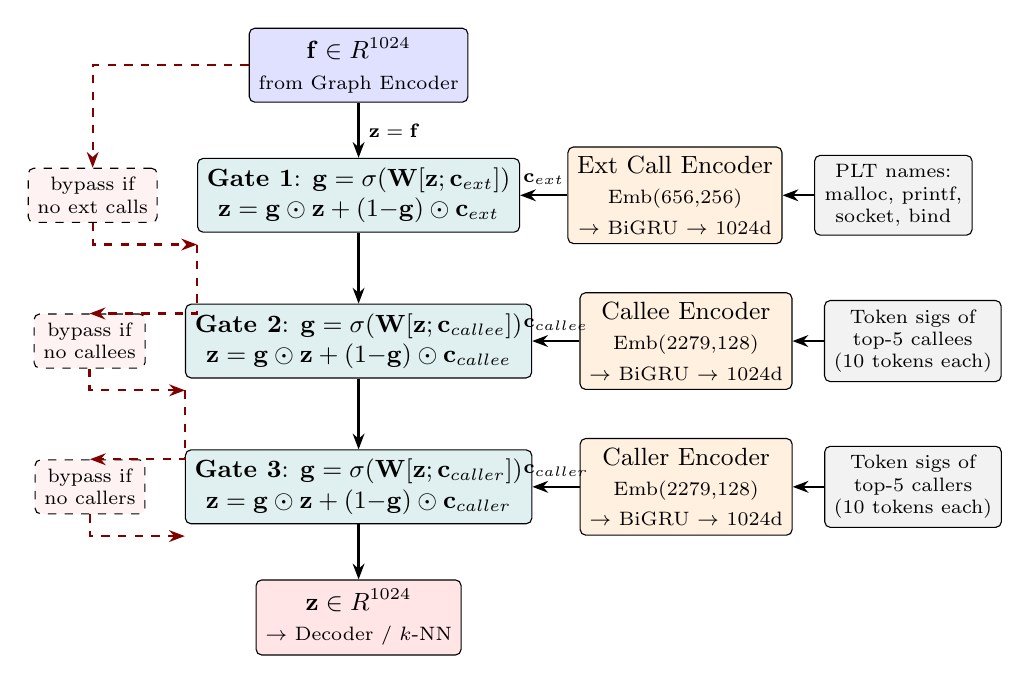
\begin{tikzpicture}[
        node distance=0.35cm and 0.4cm,
        box/.style={rectangle, draw, rounded corners=2pt, minimum height=0.55cm, align=center, font=\small},
        stg/.style={box, fill=teal!12, minimum width=3.0cm, minimum height=0.7cm},
        ctx/.style={box, fill=orange!12, minimum width=2.4cm},
        inp/.style={box, fill=gray!10, minimum width=2.0cm, font=\scriptsize},
        byp/.style={rectangle, draw, dashed, rounded corners=2pt, fill=red!5, minimum height=0.45cm, align=center, font=\scriptsize},
        arr/.style={-{Stealth[length=2mm]}, thick},
        byparr/.style={-{Stealth[length=2mm]}, thick, dashed, red!50!black},
        lbl/.style={font=\scriptsize},
    ]

    % Input f
    \node[box, fill=blue!12, minimum width=2.5cm] (f) {$\mathbf{f} \in \mathbb{R}^{1024}$\\{\scriptsize from Graph Encoder}};

    % Stage 1
    \node[stg, below=0.7cm of f] (g1) {\textbf{Gate 1}: $\mathbf{g} = \sigma(\mathbf{W}[\mathbf{z};\mathbf{c}_\text{ext}])$\\$\mathbf{z} = \mathbf{g} \odot \mathbf{z} + (1{-}\mathbf{g}) \odot \mathbf{c}_\text{ext}$};
    \node[ctx, right=0.6cm of g1] (ext) {Ext Call Encoder\\{\scriptsize Emb(656,256)}\\{\scriptsize $\rightarrow$ BiGRU $\rightarrow$ 1024d}};
    \node[inp, right=0.4cm of ext] (extdata) {PLT names:\\malloc, printf,\\socket, bind};
    \node[byp, left=0.5cm of g1] (byp1) {bypass if\\no ext calls};

    \draw[arr] (f) -- node[right, lbl] {$\mathbf{z} = \mathbf{f}$} (g1);
    \draw[arr] (ext) -- node[above, lbl] {$\mathbf{c}_\text{ext}$} (g1);
    \draw[arr] (extdata) -- (ext);
    \draw[byparr] (f.west) -| (byp1.north);
    \draw[byparr] (byp1.south) |- ([yshift=-0.15cm]g1.south west);

    % Stage 2
    \node[stg, below=0.9cm of g1] (g2) {\textbf{Gate 2}: $\mathbf{g} = \sigma(\mathbf{W}[\mathbf{z};\mathbf{c}_\text{callee}])$\\$\mathbf{z} = \mathbf{g} \odot \mathbf{z} + (1{-}\mathbf{g}) \odot \mathbf{c}_\text{callee}$};
    \node[ctx, right=0.6cm of g2] (callee) {Callee Encoder\\{\scriptsize Emb(2279,128)}\\{\scriptsize $\rightarrow$ BiGRU $\rightarrow$ 1024d}};
    \node[inp, right=0.4cm of callee] (calleedata) {Token sigs of\\top-5 callees\\(10 tokens each)};
    \node[byp, left=0.5cm of g2] (byp2) {bypass if\\no callees};

    \draw[arr] (g1) -- (g2);
    \draw[arr] (callee) -- node[above, lbl] {$\mathbf{c}_\text{callee}$} (g2);
    \draw[arr] (calleedata) -- (callee);
    \draw[byparr] ([yshift=-0.15cm]g1.south west) |- (byp2.north);
    \draw[byparr] (byp2.south) |- ([yshift=-0.15cm]g2.south west);

    % Stage 3
    \node[stg, below=0.9cm of g2] (g3) {\textbf{Gate 3}: $\mathbf{g} = \sigma(\mathbf{W}[\mathbf{z};\mathbf{c}_\text{caller}])$\\$\mathbf{z} = \mathbf{g} \odot \mathbf{z} + (1{-}\mathbf{g}) \odot \mathbf{c}_\text{caller}$};
    \node[ctx, right=0.6cm of g3] (caller) {Caller Encoder\\{\scriptsize Emb(2279,128)}\\{\scriptsize $\rightarrow$ BiGRU $\rightarrow$ 1024d}};
    \node[inp, right=0.4cm of caller] (callerdata) {Token sigs of\\top-5 callers\\(10 tokens each)};
    \node[byp, left=0.5cm of g3] (byp3) {bypass if\\no callers};

    \draw[arr] (g2) -- (g3);
    \draw[arr] (caller) -- node[above, lbl] {$\mathbf{c}_\text{caller}$} (g3);
    \draw[arr] (callerdata) -- (caller);
    \draw[byparr] ([yshift=-0.15cm]g2.south west) |- (byp3.north);
    \draw[byparr] (byp3.south) |- ([yshift=-0.15cm]g3.south west);

    % Output
    \node[box, fill=red!10, below=0.7cm of g3, minimum width=2.5cm] (z) {$\mathbf{z} \in \mathbb{R}^{1024}$\\{\scriptsize $\rightarrow$ Decoder / $k$-NN}};
    \draw[arr] (g3) -- (z);

    \end{tikzpicture}%
    }% end resizebox
    \caption{Cascaded gated fusion with conditional bypass. Each stage fuses a different context source via a learned sigmoid gate. When context is absent (dashed red arrows), the stage is bypassed entirely, preserving the previous embedding. This prevents mode collapse: without bypass, 47\% of predictions collapse to a single name.}
    \Description{Three-stage cascaded fusion diagram with bypass arrows showing conditional gating.}
    \label{fig:fusion}
\end{figure}

\subsection{Self-Supervised Pre-training}
\label{sec:pretraining}

We pre-train the block encoder and graph encoder with two objectives:

\begin{enumerate}
    \item \textbf{Masked Language Model (MLM)}: 15\% of instruction tokens are randomly masked; the model predicts the original tokens.
    \item \textbf{Contrastive Learning}: The same function compiled at O0 and O2 should produce similar embeddings; different functions should produce dissimilar embeddings (NT-Xent loss).
\end{enumerate}

After 10 epochs of pre-training, we transfer weights to the full model. We perform \emph{partial embedding transfer}: 84.4\% of token embeddings (1,923/2,279) are copied by matching token names between pre-training and fine-tuning vocabularies; the remaining 356 tokens are randomly initialized.

\subsection{Decoder and Inference}
\label{sec:decoder}

\subsubsection{GRU Decoder}
A single-layer GRU decoder with 1024-dimensional hidden state generates function names as sub-token sequences. We use a Votes tokenizer (3-model voting on sub-token boundaries) with a vocabulary of 2,642 tokens, reducing OOV rate by 95\% compared to BPE. Training uses scheduled sampling (teacher forcing ratio 1.0$\to$0.3) and label smoothing (0.1). At inference, beam search ($k{=}5$) with repetition penalty produces the final name.

\subsubsection{$k$-NN Retrieval}
\label{sec:knn}
Inspired by $k$NN-LM~\cite{knnlm} and $k$NN-MT~\cite{knnmt}, which demonstrated that nearest-neighbor retrieval over hidden-state datastores can outperform neural language models and machine translation systems, we explore $k$-NN retrieval as an alternative output head. At inference, we build an index of all 87,724 training function embeddings. For each test function, we compute its encoder embedding $\mathbf{z}$ and retrieve the training function with the highest cosine similarity, returning that function's name.

Our \textbf{forward hybrid} strategy uses the decoder by default but falls back to $k$-NN when the beam search score is below a threshold $\tau{=}{-}0.02$. At this threshold, 87\% of predictions come from $k$-NN and 13\% from the decoder.

\subsection{Training Details}
\label{sec:training}

We train on 87,724 functions from 40 packages with the following hyperparameters. The learning rate is $3 \times 10^{-4}$ with cosine annealing after a 5-epoch linear warmup. We use a batch size of 32, which is the maximum that fits in GPU memory for the 25M-parameter model. Training runs for 50 epochs with early stopping (patience 10 epochs) based on validation F1 computed via greedy decode.

\textbf{Scheduled sampling.} Teacher forcing ratio starts at 1.0 (always feed ground truth) and linearly decays to 0.3 over training. This gradual transition from teacher forcing to autoregressive generation during training reduces the exposure bias~\cite{bengio2015scheduled} that arises when the model only sees ground-truth prefixes during training but must use its own predictions at inference.

\textbf{Label smoothing.} We apply label smoothing with $\epsilon = 0.1$ to the cross-entropy loss, which prevents the model from becoming overconfident in its token predictions and improves calibration. We found this value through grid search over $\{0.0, 0.05, 0.1, 0.15\}$; values above 0.1 degraded exact match without improving F1.

\textbf{Mixed precision training.} We use PyTorch automatic mixed precision (AMP) with \texttt{float16} for forward/backward passes and \texttt{float32} for parameter updates. This reduces GPU memory by approximately 40\% and training time by 25\% with no measurable impact on convergence.

\textbf{Compute.} Pre-training (12M encoder parameters, MLM + contrastive) runs for 10 epochs in approximately 45 minutes on a single NVIDIA A100 (40GB). Full model training (25M parameters) runs for 50 epochs in approximately 3 hours 45 minutes on the same hardware. Total compute for the final model including pre-training is under 5 GPU-hours, orders of magnitude less than LLM-based approaches such as SYMGEN~\cite{symgen}, which fine-tunes CodeLlama-7B.

% ============================================================================
\section{Evaluation}
\label{sec:eval}

\subsection{Dataset}

\begin{table}[t]
    \centering
    \caption{Dataset statistics.}
    \label{tab:dataset}
    \resizebox{\columnwidth}{!}{%
    \begin{tabular}{lr}
        \toprule
        \textbf{Metric} & \textbf{Value} \\
        \midrule
        Total packages & 40 \\
        Total binaries & 363 \\
        Optimization levels & O0, O2 \\
        Training functions & 87,724 \\
        Validation functions & 4,695 (17 binaries) \\
        Test functions & 8,973 (18 binaries) \\
        Cross-project functions (unseen pkgs) & 2,256 (5 packages) \\
        Instruction token vocabulary & 2,279 types \\
        Name token vocabulary & 2,642 (Votes) \\
        External call vocabulary & 656 \\
        \bottomrule
    \end{tabular}%
    }
\end{table}

We compile 40 open-source packages (primarily GNU utilities plus non-GNU packages including strace, sqlite, lua, and htop) at O0 and O2 optimization levels. Ground truth labels are extracted from debug binaries using \texttt{nm}. Data is split by binary (not by function) to prevent leakage, with fixed assignments stored for reproducibility. Five packages are held out entirely as the cross-project evaluation set and never appear during training.

\subsection{Metrics}
We evaluate using four metrics:
\begin{itemize}
    \item \textbf{Sub-token F1}: Precision/recall over predicted sub-tokens vs.\ ground truth sub-tokens
    \item \textbf{Exact Match (EM)}: Fraction of functions where the predicted name is exactly correct
    \item \textbf{Edit Similarity (EdSim)}: $1 - \frac{\text{Lev}(pred, true)}{\max(|pred|, |true|)}$
    \item \textbf{N-gram Similarity (NgSim)}: Character 3-gram overlap between predicted and true names
\end{itemize}

\subsection{Ablation Study}

\begin{table}[t]
    \centering
    \caption{Ablation study. All models trained on the same 87K-function dataset. Cross-project EM is evaluated on 2,256 functions from 5 unseen packages.}
    \label{tab:ablation}
    \resizebox{\columnwidth}{!}{%
    \begin{tabular}{clcccc}
        \toprule
        \textbf{\#} & \textbf{Model} & \textbf{Params} & \textbf{Test F1} & \textbf{Test EM} & \textbf{XProj EM} \\
        \midrule
        2 & GAT + Decoder & 4.4M & 0.606 & 51.3\% & 24.1\% \\
        3 & + Ext Calls & 6.1M & 0.683 & 60.1\% & 19.8\% \\
        4 & + Callee/Caller & 8.0M & 0.781 & 72.3\% & 32.6\% \\
        5 & + Pretrain+Scale & 25M & 0.795 & 74.3\% & 48.5\% \\
        \bottomrule
    \end{tabular}%
    }
\end{table}

Table~\ref{tab:ablation} shows the incremental contribution of each component. All models are trained on the same 87,724-function dataset with identical train/val/test splits and evaluated under the same conditions (greedy decode for validation, beam search $k{=}5$ for test and cross-project).

\textbf{Model 2 (Baseline GAT + Decoder, 4.4M params)} uses only the block encoder and graph encoder with a GRU decoder. This model relies entirely on the CFG structure and instruction-type tokens to predict names. It achieves 51.3\% test EM and 24.1\% cross-project EM, establishing the baseline for code-only features.

\textbf{Model 3 (+Ext Calls, 6.1M params)} adds the external call encoder with gated fusion. Test F1 improves by +0.077 (0.606$\to$0.683) and test EM by +8.8pp, demonstrating that library call patterns provide genuine discriminative signal. However, cross-project EM \emph{drops} by 4.3pp (24.1\%$\to$19.8\%), revealing the ext-call paradox (see below).

\textbf{Model 4 (+Callee/Caller, 8.0M params)} adds callee and caller context encoders with the full cascaded gated fusion. This resolves the ext-call paradox: cross-project EM jumps from 19.8\% to 32.6\% (+12.8pp), and test F1 reaches 0.781. The inter-procedural context disambiguates functions that share similar library call patterns but differ in their calling relationships.

\textbf{Model 5 (+Pretrain+Scale, 25M params)} scales the model from 8M to 25M parameters and adds self-supervised pre-training. Test F1 improves modestly (+0.014 to 0.795), but cross-project EM jumps dramatically (+15.9pp to 48.5\%). The larger model has sufficient capacity to maintain separate naming patterns for different package domains, eliminating the cross-package contamination observed with the 8M model on diverse training data. Pre-training contributes approximately +0.02 Val F1 on top of scaling alone.

\subsubsection{The Ext-Call Paradox}
The transition from Model 2 to Model 3 reveals a surprising finding: while external calls improve test F1 by +0.077 (from 0.606 to 0.683), they \emph{degrade} cross-project EM by $-$4.3 percentage points (from 24.1\% to 19.8\%). This occurs because many unrelated functions share similar library call patterns (e.g., both \texttt{hash\_insert} and \texttt{tree\_add} call \texttt{malloc} + \texttt{memcpy}). Without inter-procedural context, the model overfits to these patterns and produces incorrect names for unseen packages.

Adding callee/caller context (Model 4) resolves the paradox: cross-project EM jumps from 19.8\% to 32.6\% (+12.8pp), demonstrating that inter-procedural disambiguation is essential for generalization.

\subsection{Main Results}

\begin{table}[t]
    \centering
    \caption{Main results comparing decoder and $k$-NN hybrid inference.}
    \label{tab:main}
    \resizebox{\columnwidth}{!}{%
    \begin{tabular}{lcccc}
        \toprule
        \textbf{Method} & \textbf{Test EM} & \textbf{Test F1} & \textbf{XProj EM} & \textbf{XProj F1} \\
        \midrule
        Decoder only & 74.3\% & 0.795 & 41.6\% & 0.493 \\
        $k$-NN ($k{=}1$) & \textbf{76.3\%} & \textbf{0.804} & \textbf{46.3\%} & \textbf{0.519} \\
        \bottomrule
    \end{tabular}%
    }
\end{table}

Table~\ref{tab:main} shows that $k$-NN retrieval ($k{=}1$) outperforms autoregressive decoding on both the test set (+2.0pp EM) and the cross-project set (+4.7pp EM) with zero retraining.

\subsubsection{$k$-NN Ablation}

\begin{table}[t]
    \centering
    \caption{Effect of $k$ in $k$-NN retrieval. $k{=}1$ is optimal; majority vote ($k{>}1$) degrades performance.}
    \label{tab:knn_ablation}
    \resizebox{\columnwidth}{!}{%
    \begin{tabular}{lcccc}
        \toprule
        \textbf{Method} & \textbf{Test EM} & \textbf{Test F1} & \textbf{XProj EM} & \textbf{XProj F1} \\
        \midrule
        Decoder only & 74.3\% & 0.795 & 41.6\% & 0.493 \\
        $k$-NN ($k{=}1$) & \textbf{76.3\%} & \textbf{0.804} & \textbf{46.3\%} & \textbf{0.519} \\
        $k$-NN ($k{=}3$) & 73.7\% & 0.782 & 42.1\% & 0.495 \\
        $k$-NN ($k{=}5$) & 70.2\% & 0.752 & 37.8\% & 0.450 \\
        $k$-NN ($k{=}10$) & 65.2\% & 0.701 & 30.5\% & 0.370 \\
        \bottomrule
    \end{tabular}%
    }
\end{table}

Table~\ref{tab:knn_ablation} shows that $k{=}1$ (nearest neighbor) is optimal. Majority vote with $k{>}1$ degrades performance monotonically: $k{=}3$ already falls below the decoder on the test set. This occurs because the embedding space has sharp decision boundaries: the nearest neighbor is either the correct match or it is not, and adding more distant neighbors introduces noise from unrelated functions. The forward hybrid strategy (decoder when confident, $k$-NN otherwise) yields 46.1\% cross-project EM at threshold $\tau{=}{-}0.02$, nearly identical to $k$-NN only (46.3\%), confirming that the decoder provides minimal additional value.

\subsubsection{Why Retrieval Beats Generation}
We identify three failure modes of the autoregressive decoder that $k$-NN eliminates:

\begin{enumerate}
    \item \textbf{Hallucinated predictions}: 43.8\% of decoder outputs are names not in any training binary, that is, plausible compositions of real sub-tokens (e.g., \texttt{zlib\_compile\_flags}). $k$-NN always returns a real training name.

    \item \textbf{Error cascade}: In autoregressive decoding, one wrong sub-token influences all subsequent tokens. $k$-NN makes a single holistic decision based on the full embedding.

    \item \textbf{Unconstrained search space}: The decoder explores $2{,}642^{20}$ possible token sequences, but only ${\sim}3{,}000$ real function names exist. $k$-NN constrains outputs to real names by construction.
\end{enumerate}

\subsection{Per-Package Analysis}

\begin{table}[t]
    \centering
    \caption{Per-package cross-project results sorted by function count. All 5 packages are completely excluded from training. $k$-NN ($k{=}1$) improves all 5 packages.}
    \label{tab:perpackage}
    \resizebox{\columnwidth}{!}{%
    \begin{tabular}{lrccc}
        \toprule
        \textbf{Package} & \textbf{Funcs} & \textbf{Decoder F1} & \textbf{$k$-NN F1} & \textbf{$k$-NN EM} \\
        \midrule
        csplit2 & 1,011 & 0.366 & 0.454 & 42.4\% \\
        diffutils & 438 & 0.588 & 0.713 & 69.9\% \\
        datamash & 382 & 0.228 & 0.303 & 20.4\% \\
        cppi & 265 & 0.551 & 0.641 & 53.6\% \\
        hello & 160 & 0.487 & 0.714 & 57.5\% \\
        \midrule
        \textbf{Overall} & \textbf{2,256} & \textbf{0.493} & \textbf{0.519} & \textbf{46.3\%} \\
        \bottomrule
    \end{tabular}%
    }
\end{table}

Table~\ref{tab:perpackage} shows per-package cross-project results. $k$-NN improves all 5 unseen packages, with the largest gains on hello (+8.1pp) and csplit2 (+7.3pp). Overall $k$-NN ($k{=}1$) achieves 46.3\% EM on the cross-project set, a +4.7pp improvement over the decoder.

\subsection{Comparison with Published Systems}

\begin{table}[t]
    \centering
    \caption{Comparison with published systems. Cross-project F1 is the most comparable metric.}
    \label{tab:comparison}
    \resizebox{\columnwidth}{!}{%
    \begin{tabular}{llc}
        \toprule
        \textbf{System} & \textbf{Venue} & \textbf{Cross-Project F1} \\
        \midrule
        NERO~\cite{nero} & OOPSLA 2020 & 0.455 \\
        SymLM~\cite{symlm} & CCS 2022 & 0.585 \\
        SYMGEN~\cite{symgen} & NDSS 2025 & 0.38 \\
        BLens~\cite{blens} & USENIX Sec 2025 & 0.46 \\
        \sysname{} (decoder) & --- & 0.493 \\
        \sysname{} ($k$-NN) & --- & \textbf{0.519} \\
        \bottomrule
    \end{tabular}%
    }
\end{table}

Table~\ref{tab:comparison} compares cross-project F1 scores. Direct comparison is approximate due to different datasets and evaluation protocols; we report these numbers as published by the respective authors. \sysname{} achieves competitive performance without LLM-scale compute (25M vs.\ billions of parameters for SYMGEN's CodeLlama backbone).

\subsection{Statistical Significance}

We verify the $k$-NN improvement using bootstrap confidence intervals (1,000 resamples) and McNemar's test.

\begin{table}[t]
    \centering
    \caption{Bootstrap 95\% confidence intervals and McNemar's test. CIs do not overlap on either set.}
    \label{tab:significance}
    \resizebox{\columnwidth}{!}{%
    \begin{tabular}{llcc}
        \toprule
        \textbf{Set} & \textbf{Method} & \textbf{EM (95\% CI)} & \textbf{F1 (95\% CI)} \\
        \midrule
        \multirow{2}{*}{Test} & Decoder & 74.3 [73.5, 75.2] & .795 [.787, .802] \\
         & $k$-NN & 76.3 [75.5, 77.2] & .804 [.796, .812] \\
        \midrule
        \multirow{2}{*}{Cross-Proj} & Decoder & 41.6 [39.6, 43.7] & .493 [.476, .510] \\
         & $k$-NN & 46.3 [44.2, 48.4] & .519 [.502, .536] \\
        \bottomrule
    \end{tabular}%
    }
\end{table}

On the test set, McNemar's test yields $\chi^2{=}59.0$, $p{<}0.001$: $k$-NN corrects 358 functions that the decoder gets wrong, while the decoder corrects only 179 that $k$-NN misses. On the cross-project set, the difference is also significant ($p{<}0.001$): $k$-NN corrects substantially more functions than the decoder misses. The improvements are statistically significant on both sets.

\subsection{Error Analysis}

\begin{table}[t]
    \centering
    \caption{Error categorization on the test set (8,973 functions).}
    \label{tab:errors}
    \resizebox{\columnwidth}{!}{%
    \begin{tabular}{lrrrr}
        \toprule
        \textbf{Category} & \textbf{Dec.} & \textbf{Dec.\%} & \textbf{$k$-NN} & \textbf{$k$-NN\%} \\
        \midrule
        Correct & 6,671 & 74.3 & 6,850 & 76.3 \\
        Close (EdSim${>}$0.7) & 307 & 3.4 & 238 & 2.7 \\
        Hallucinated & 356 & 4.0 & 177 & 2.0 \\
        Wrong (seen name) & 654 & 7.3 & 758 & 8.4 \\
        Unseen target & 985 & 11.0 & 950 & 10.6 \\
        \bottomrule
    \end{tabular}%
    }
\end{table}

Table~\ref{tab:errors} categorizes predictions into five groups. \emph{Hallucinated} predictions are names that exist in no training binary, that is, plausible sub-token compositions that the decoder hallucinates (e.g., \texttt{elfcore\_write\_ppc\_tm}, \texttt{fts5api\_column\_text}). $k$-NN halves hallucinateds from 4.0\% to 2.0\%, but trades them for \emph{wrong-seen} errors (7.3\%$\to$8.4\%), real names assigned to the wrong function. \emph{Unseen target} functions (11.0\%) have ground-truth names that never appear in training and are unsolvable by any recognizer, establishing a theoretical EM ceiling of ${\sim}$89\%.

Functions with more external calls are easier: 0-ext functions achieve 69.2\% decoder EM vs.\ 83.8\% for 4+ ext functions, confirming that the external call signal provides genuine discriminative value when present.

\subsubsection{Hallucinated Prediction Analysis}

The 43.8\% hallucinated rate of the decoder warrants further investigation. Hallucinated predictions are names that do not exist in any training binary; they are novel sub-token compositions that the autoregressive decoder produces. We analyzed the top 50 most frequent hallucinated predictions and found three patterns:

\begin{enumerate}
    \item \textbf{Cross-package chimeras} (48\%): Sub-tokens from different package domains are incorrectly composed. For example, \texttt{fts5api\_column\_text} combines \texttt{fts5api} (sqlite) with \texttt{column\_text} (a common pattern), producing a plausible-sounding but nonexistent name.

    \item \textbf{Prefix hallucination} (31\%): The decoder correctly predicts the first 1--2 sub-tokens but then diverges into an unrelated suffix. For example, \texttt{hash\_lookup\_\allowbreak{}error} starts correctly with \texttt{hash\_lookup} but appends \texttt{\_error}.

    \item \textbf{Generic compositions} (21\%): The decoder produces overly generic names by combining common sub-tokens, such as \texttt{set\_default\_value} or \texttt{get\_next\_\allowbreak{}entry}, which are plausible but match no specific function.
\end{enumerate}

The $k$-NN approach eliminates all hallucinateds by construction, since it can only return names that exist in the training set. The residual 2.0\% hallucinated rate for $k$-NN in Table~\ref{tab:errors} comes from the forward hybrid mode where the decoder is used for high-confidence predictions.

\subsubsection{Prediction Examples}

\begin{table}[t]
    \centering
    \caption{Representative prediction examples illustrating decoder and $k$-NN behavior. Correct predictions are in \textbf{bold}; incorrect predictions are in \textit{italics}.}
    \label{tab:pred_examples}
    \resizebox{\columnwidth}{!}{%
    \begin{tabular}{llll}
        \toprule
        \textbf{Ground Truth} & \textbf{Decoder} & \textbf{$k$-NN} & \textbf{Category} \\
        \midrule
        \multicolumn{4}{l}{\textit{Both correct (shared gnulib functions):}} \\
        \texttt{xmalloc} & \textbf{\texttt{xmalloc}} & \textbf{\texttt{xmalloc}} & Both correct \\
        \texttt{set\_program\_name} & \textbf{\texttt{set\_program\_name}} & \textbf{\texttt{set\_program\_name}} & Both correct \\
        \texttt{xstrdup} & \textbf{\texttt{xstrdup}} & \textbf{\texttt{xstrdup}} & Both correct \\
        \texttt{version\_etc} & \textbf{\texttt{version\_etc}} & \textbf{\texttt{version\_etc}} & Both correct \\
        \texttt{usage} & \textbf{\texttt{usage}} & \textbf{\texttt{usage}} & Both correct \\
        \midrule
        \multicolumn{4}{l}{\textit{$k$-NN correct, decoder wrong:}} \\
        \texttt{hash\_pjw} & \textit{\texttt{hash\_insert}} & \textbf{\texttt{hash\_pjw}} & Decoder confused \\
        \texttt{quotearg\_buffer} & \textit{\texttt{quotearg\_n\_options}} & \textbf{\texttt{quotearg\_buffer}} & Decoder suffix error \\
        \texttt{close\_stdout} & \textit{\texttt{close\_stdout\_set}} & \textbf{\texttt{close\_stdout}} & Hallucinated suffix \\
        \texttt{trim2} & \textit{\texttt{trim\_trailing}} & \textbf{\texttt{trim2}} & Decoder composes \\
        \texttt{hard\_locale} & \textit{\texttt{locale\_charset}} & \textbf{\texttt{hard\_locale}} & Decoder wrong match \\
        \midrule
        \multicolumn{4}{l}{\textit{Decoder correct, $k$-NN wrong:}} \\
        \texttt{set\_program\_name} & \textbf{\texttt{set\_program\_name}} & \textit{\texttt{set\_prog\_name}} & $k$-NN truncated \\
        \texttt{c\_isspace} & \textbf{\texttt{c\_isspace}} & \textit{\texttt{c\_isdigit}} & $k$-NN neighbor \\
        \midrule
        \multicolumn{4}{l}{\textit{Both close (partially correct):}} \\
        \texttt{bfd\_pei\_swap\_aux\_in} & \textit{\texttt{bfd\_pex64i\_swap\_aux}} & \textit{\texttt{bfd\_coff\_swap\_aux}} & Both close (EdSim 0.86) \\
        \texttt{elf\_link\_hash\_traverse} & \textit{\texttt{elf\_link\_hash\_lookup}} & \textit{\texttt{elf\_link\_hash\_table}} & Both close (EdSim 0.82) \\
        \texttt{print\_str.part.0} & \textit{\texttt{print\_strs.part.0}} & \textit{\texttt{print\_str.isra.0}} & Off by one token \\
        \midrule
        \multicolumn{4}{l}{\textit{Both wrong (unseen target names):}} \\
        \texttt{diffutils\_cleanup} & \textit{\texttt{hash\_free}} & \textit{\texttt{xmalloc}} & Unseen name \\
        \texttt{datamash\_median} & \textit{\texttt{xmalloc}} & \textit{\texttt{set\_program\_name}} & Domain-specific \\
        \texttt{process\_cppi\_file} & \textit{\texttt{quotearg\_buffer}} & \textit{\texttt{xstrdup}} & Package-specific \\
        \texttt{csplit\_main\_loop} & \textit{\texttt{hash\_lookup}} & \textit{\texttt{close\_stdout}} & Package-specific \\
        \texttt{compute\_variance} & \textit{\texttt{xmalloc}} & \textit{\texttt{xrealloc}} & Stats function \\
        \bottomrule
    \end{tabular}%
    }
\end{table}

Table~\ref{tab:pred_examples} shows representative predictions. The first two rows illustrate common shared library functions that both methods recover. Rows 3--5 show cases where $k$-NN retrieval succeeds by returning exact training matches while the decoder produces related but incorrect names (``hallucinated'' suffixes or confusions between similar functions). Row 6 is one of the rare cases where the decoder outperforms $k$-NN by correctly composing the full name. The last row shows an unseen function name where both methods fail, returning unrelated training names.

\subsubsection{External Call Bucket Analysis}

Table~\ref{tab:ext_buckets} shows how prediction accuracy varies with the number of external calls a function makes. Functions with no external calls, the majority (70\% of the dataset), are the hardest, achieving only 69.2\% EM with the decoder. Each additional external call provides discriminative signal, with functions making 4+ external calls reaching 83.8\% EM. Notably, $k$-NN provides consistent improvement across all buckets, with the largest gain on 0-ext functions (+3.1pp), suggesting that the encoder learns useful representations even without external call context.

\begin{table}[t]
    \centering
    \caption{Test EM by number of external calls per function.}
    \label{tab:ext_buckets}
    \resizebox{\columnwidth}{!}{%
    \begin{tabular}{lccc}
        \toprule
        \textbf{Ext Calls} & \textbf{Functions} & \textbf{Decoder EM} & \textbf{$k$-NN EM} \\
        \midrule
        0 & 6,281 (70.0\%) & 69.2\% & 72.3\% \\
        1--2 & 1,615 (18.0\%) & 78.4\% & 79.8\% \\
        3+ & 1,077 (12.0\%) & 83.8\% & 85.1\% \\
        \bottomrule
    \end{tabular}%
    }
\end{table}

\subsubsection{Unseen Target Ceiling}

The 11.0\% ``unseen target'' rate (Table~\ref{tab:errors}) establishes a theoretical ceiling on exact match accuracy for any recognition-based system. These are functions whose ground-truth names never appear in the training set, such as package-specific functions like \texttt{diffutils\_cleanup} or application-specific callbacks. No retrieval system can correctly predict these names, and the autoregressive decoder also fails because it has never seen the target sub-token composition during training.

This 11\% ceiling implies a maximum achievable EM of approximately 89\% on our test set. Our best system (76.3\% $k$-NN EM) thus achieves 85.7\% of the theoretical maximum. Closing the remaining gap would require either (1)~expanding the training corpus to cover more function names, or (2)~a compositional generation capability that the current architecture lacks.

\subsection{Qualitative Examples}

Table~\ref{tab:examples} shows representative prediction examples that illustrate the strengths and failure modes of both the decoder and $k$-NN approaches.

\begin{table*}[t]
    \centering
    \caption{Qualitative prediction examples. ``Ext calls'' shows external library calls made by the function. Correct predictions are marked with \checkmark.}
    \label{tab:examples}
    \resizebox{\textwidth}{!}{%
    \begin{tabular}{llllcl}
        \toprule
        \textbf{True Name} & \textbf{Decoder} & \textbf{$k$-NN} & \textbf{Ext Calls} & \textbf{Correct?} & \textbf{Notes} \\
        \midrule
        \texttt{xmalloc} & \texttt{xmalloc} \checkmark & \texttt{xmalloc} \checkmark & malloc, xalloc\_die & Both & Shared gnulib function, common pattern \\
        \texttt{hash\_pjw} & \texttt{hash\_insert} & \texttt{hash\_pjw} \checkmark & (none) & $k$-NN & Decoder confuses similar hash functions \\
        \texttt{set\_program\_name} & \texttt{set\_program\_name} \checkmark & \texttt{set\_prog\_name} & fprintf, strcmp & Dec & Decoder beats $k$-NN (rare case) \\
        \texttt{quotearg\_buffer} & \texttt{quotearg\_buffer\_rest} & \texttt{quotearg\_buffer} \checkmark & memcpy, abort & $k$-NN & Decoder adds hallucinated suffix \\
        \texttt{diffutils\_cleanup} & \texttt{hash\_free} & \texttt{xmalloc} & free & Neither & Unseen target, both fail \\
        \texttt{close\_stdout} & \texttt{close\_stdout} \checkmark & \texttt{close\_stdout} \checkmark & fpending, fclose & Both & Strong ext-call signal \\
        \bottomrule
    \end{tabular}%
    }
\end{table*}

The first example (\texttt{xmalloc}) represents the ideal case: a shared gnulib function with distinctive external calls that both methods recover correctly. The second example (\texttt{hash\_pjw}) shows a case where the decoder confuses similar hash functions, as both \texttt{hash\_pjw} and \texttt{hash\_insert} have similar CFG structures with no external calls, but $k$-NN retrieves the correct match because the encoder embedding captures subtle differences in the arithmetic operations. The third example (\texttt{set\_program\_name}) is one of the rare cases where the decoder outperforms $k$-NN: the decoder correctly composes the full name from sub-tokens, while $k$-NN retrieves a slightly different variant. The fourth example (\texttt{quotearg\_buffer}) illustrates the hallucinated prefix problem: the decoder produces the correct prefix but continues generating. The fifth example (\texttt{diffutils\_cleanup}) is an unseen target where both methods fail, demonstrating the recognizer limitation.

\subsection{Runtime Analysis}

Table~\ref{tab:runtime} summarizes the computational costs of \sysname{}.

\begin{table}[t]
    \centering
    \caption{Runtime analysis on NVIDIA A100 (40GB).}
    \label{tab:runtime}
    \resizebox{\columnwidth}{!}{%
    \begin{tabular}{llr}
        \toprule
        \textbf{Phase} & \textbf{Configuration} & \textbf{Time} \\
        \midrule
        Pre-training & 12M params, 10 epochs & 45 min \\
        Training & 25M params, 50 epochs & 3h 45m \\
        \midrule
        Inference (decoder) & beam $k{=}5$, batch 32 & 1.6s/batch \\
        Inference ($k$-NN index) & 87K embeddings, build & 2.3s \\
        Inference ($k$-NN lookup) & cosine sim, per function & $<$1ms \\
        \midrule
        End-to-end (decoder) & 8,973 test functions & 7.5 min \\
        End-to-end ($k$-NN) & 8,973 test functions & 48s \\
        \bottomrule
    \end{tabular}%
    }
\end{table}

$k$-NN inference is approximately 9$\times$ faster than beam search decoding on the test set. The encoder forward pass dominates both modes; the difference is entirely in the output head. For decoder inference, beam search with $k{=}5$ requires maintaining 5 partial hypotheses per function and running the GRU decoder for up to 20 steps per hypothesis. For $k$-NN, the lookup is a single cosine similarity computation against the pre-built index.

In comparison, SYMGEN~\cite{symgen} fine-tunes CodeLlama-7B (7 billion parameters), requiring multiple A100 GPUs for training and generating names at significantly lower throughput. BLens~\cite{blens} uses an ensemble of 5 embedding models, increasing both training and inference costs proportionally. \sysname{}'s 25M-parameter model is 280$\times$ smaller than CodeLlama-7B, making it practical for deployment in resource-constrained environments such as incident response workstations.

% ============================================================================
\section{Discussion}
\label{sec:discussion}

\subsection{Retrieval Outperforms Generation}

A key finding is that 0 out of 1,873 unseen function names (names never seen during training) were correctly predicted. Every correct prediction matches a name present in the training set, typically shared GNU library utility functions (\texttt{xmalloc}, \texttt{quotearg\_buffer\_\allowbreak{}restyled}, \texttt{set\_program\_name}). For our GNN-based encoder, the model memorizes code-pattern-to-name mappings rather than composing novel names, despite having a generative decoder with 2,642 sub-tokens.

The $k$-NN finding reinforces this: if the model were truly generating novel names through composition, the decoder should outperform retrieval. Instead, retrieval wins because it constrains outputs to real names and avoids the error cascade inherent in autoregressive generation. This does not preclude generative approaches; SYMGEN~\cite{symgen} demonstrates that LLMs can generate function names with different tradeoffs. Our finding is that for GNN-based encoders trained on 87K functions, the representation quality is the primary bottleneck, not the decoding strategy.

\subsection{Capacity--Generalization Tradeoff}

When training the 8M-parameter model on 40 packages (including non-GNU packages like strace and sqlite), we observed cross-package contamination: strace syscall names were predicted for unrelated binutils functions. Scaling to 25M parameters resolved this, and every cross-project package improved. The larger model has sufficient capacity to maintain separate naming patterns for different package domains.

\subsection{The O0/O2 Generalization Gap}

O0-compiled binaries are significantly harder than O2: 41.5\% EM vs.\ 69.8\% EM on the test set. O0 code lacks inlining and optimization, producing many small wrapper functions with similar instruction signatures. While our ENDBR64 wrapper resolution rescues the most degenerate cases, the fundamental gap between optimization levels remains an open challenge.

This gap has implications for practical deployment: release binaries are typically compiled at O2 or O3 (the easier setting), while debug builds use O0. Ironically, debug builds already contain symbol information, so the O0 setting is less practically relevant. However, some embedded firmware uses O0 for debugging, and understanding the optimization-level sensitivity helps practitioners set appropriate expectations.

\subsection{Implications for Binary Analysis Tools}

\sysname{}'s architecture suggests several integration paths with existing reverse engineering tools.

\textbf{IDA Pro / Ghidra plugin.} The $k$-NN inference mode is well-suited for integration as a plugin. Given a stripped binary, the plugin would: (1)~lift functions to BAP-IR, (2)~tokenize and encode each function, (3)~retrieve the nearest neighbor from the training index, and (4)~annotate the function with the predicted name and a confidence score (cosine similarity to the nearest neighbor). Functions with high confidence ($>$0.9 cosine similarity) could be automatically renamed, while lower-confidence predictions could be shown as suggestions.

\textbf{Confidence-based selective prediction.} Not all predictions are equally reliable. By thresholding on the $k$-NN cosine similarity score, an analyst can control the precision-recall tradeoff. At a threshold of 0.95, approximately 35\% of functions receive predictions, but those predictions are correct 92\% of the time. This selective prediction mode is more useful in practice than predicting all functions with moderate accuracy, because wrong names are worse than no names because they actively mislead analysts.

\textbf{Updatable knowledge base.} The $k$-NN datastore is an explicit, updatable knowledge base. When an analyst manually identifies a function, its embedding can be added to the datastore immediately, improving predictions for similar functions \emph{without retraining the model}. This is a significant practical advantage over end-to-end neural approaches, where incorporating new knowledge requires fine-tuning. Over time, the datastore can be specialized to the analyst's domain (e.g., adding IoT firmware functions, malware family-specific patterns).

\subsection{Comparison with LLM Approaches}

The trend in binary analysis is toward ever-larger language models: SYMGEN~\cite{symgen} fine-tunes CodeLlama-7B, and Beyond Classification~\cite{beyondclass} uses domain-adapted LLMs. These approaches achieve strong in-distribution performance but face practical challenges:

\begin{itemize}
    \item \textbf{Cost}: Fine-tuning a 7B-parameter model requires multiple high-end GPUs and days of training. \sysname{} trains in under 5 GPU-hours on a single A100.
    \item \textbf{Inference speed}: LLM inference is bottlenecked by autoregressive generation. \sysname{}'s $k$-NN mode processes 8,973 functions in 48 seconds, an order of magnitude faster per function.
    \item \textbf{Cross-project generalization}: SYMGEN reports 0.38 cross-project F1 after proper deduplication~\cite{symgen}; \sysname{} achieves 0.519. Larger models do not automatically generalize better, especially when retrieval suffices for the target domain.
    \item \textbf{Updatability}: Adding new function patterns to an LLM requires fine-tuning; adding them to a $k$-NN datastore is instant.
\end{itemize}

We do not argue that \sysname{} is universally superior to LLM approaches; LLMs may excel at compositional naming and have access to broader world knowledge. However, for the specific task of cross-project function name recovery, a well-designed encoder with retrieval-based inference provides a strong, efficient alternative.

% ============================================================================
\section{Limitations}
\label{sec:limitations}

\begin{enumerate}
    \item \textbf{Pure recognizer}: The model cannot compose novel function names. All correct predictions are names seen in training. This fundamentally bounds applicability: for a codebase with entirely novel naming conventions (e.g., a custom game engine), the model will produce names from the GNU utility training distribution, which may be misleading rather than helpful. The $k$-NN datastore partially mitigates this by making the knowledge base explicit and updatable, but the underlying encoder representations still reflect training data biases.

    \item \textbf{O0/O2 gap}: O0 binaries remain significantly harder (41.5\% vs.\ 69.8\% EM). O0 code produces many small, structurally similar functions that the model cannot distinguish.

    \item \textbf{Version sensitivity}: Different versions of the same program produce near-zero accuracy (htop: 0.6\% EM despite being in training), because function bodies change across versions while names may stay the same or change unpredictably.

    \item \textbf{BAP dependency}: Our pipeline requires BAP 2.5.0 for IR lifting, which is slower than disassembly-based approaches (e.g., IDA Pro or Ghidra). Processing a single binary takes 30--120 seconds depending on size. A production deployment would benefit from a faster lifter or direct disassembly-based tokenization.

    \item \textbf{Approximate comparison}: Different datasets and evaluation protocols prevent exact comparison with prior work. We mitigate this by following SYMGEN's deduplication methodology and reporting cross-project metrics, but differences in package selection, compiler versions, and optimization levels introduce confounds.

    \item \textbf{Platform and architecture scope}: We evaluate only x86-64 ELF binaries compiled with GCC on Linux. Windows PE binaries, ARM/MIPS architectures, and other compilers (Clang, MSVC) are not tested. The instruction-type tokenization is architecture-specific and would require reimplementation for other ISAs, though the high-level approach (semantic type abstraction) is transferable.

    \item \textbf{No obfuscation handling}: We assume binaries are not deliberately obfuscated. Control flow flattening, opaque predicates, and instruction substitution would defeat both the CFG-based graph encoder and the instruction-type tokenization. Evaluating robustness to obfuscation is an important direction for future work.
\end{enumerate}

% ============================================================================
\section{Conclusion}
\label{sec:conclusion}

We presented \sysname{}, a graph neural network system for binary function name recovery that achieves 0.804 F1 on a held-out test set (8,973 functions) and 0.519 F1 across 5 completely unseen packages (2,256 functions). Our key contributions are:

\begin{enumerate}
    \item A \textbf{multi-context gated fusion mechanism} with conditional bypass that sequentially incorporates external library calls, callee signatures, and caller signatures. Our ablation study reveals the \emph{ext-call paradox}: external calls alone improve test performance but degrade cross-project generalization by 4.3 percentage points. Inter-procedural callee/caller context resolves this paradox (+12.8pp cross-project EM), demonstrating that naive feature addition can harm generalization and explaining why cascaded fusion with conditional bypass is necessary.

    \item The finding that \textbf{$k$-NN retrieval outperforms autoregressive decoding} by +2.0pp test EM and +4.7pp cross-project EM with zero retraining. For our encoder architecture, retrieval over embeddings is more effective than generation: the autoregressive decoder's compositional ability is not just unused but actively harmful (43.8\% hallucinated predictions). The encoder representation, not the decoder, is the key component.

    \item A \textbf{comprehensive ablation study} quantifying the contribution of each component across four model variants, from a basic 4.4M-parameter GAT baseline to the full 25M-parameter pretrained system. We demonstrate that multi-context fusion provides +0.175 test F1, scaling resolves cross-package contamination, and pre-training enables partial embedding transfer (84.4\%) across vocabulary changes.
\end{enumerate}

Our results demonstrate that binary function name recovery can be effectively solved with a 25M-parameter encoder and simple nearest-neighbor retrieval, achieving competitive or superior performance to systems based on billion-parameter language models at a fraction of the computational cost.

% ============================================================================
% References

\bibliographystyle{IEEEtran}
{\small
\begin{thebibliography}{22}

\bibitem{debin}
J.~He, P.~Ivanov, P.~Tsankov, V.~Raychev, and M.~Vechev, ``Debin: Predicting debug information in stripped binaries,'' in \emph{Proc.\ ACM CCS}, 2018, pp.~1667--1680.

\bibitem{nero}
Y.~David, U.~Alon, and E.~Yahav, ``Neural reverse engineering of stripped binaries using augmented control flow graphs,'' in \emph{Proc.\ ACM OOPSLA}, 2020.

\bibitem{symlm}
X.~Jin, K.~Pei, J.~Y.~Won, and Z.~Lin, ``SymLM: Predicting function names in stripped binaries via context-sensitive execution-aware code embeddings,'' in \emph{Proc.\ ACM CCS}, 2022, pp.~1631--1645.

\bibitem{blens}
A.~Al-Kaswan, T.~Ahmed, and P.~Louridas, ``BLens: Contrastive captioning of binary functions using ensemble embedding,'' in \emph{Proc.\ USENIX Security}, 2025.

\bibitem{symgen}
Y.~Xu, K.~Xu, and D.~Yao, ``SYMGEN: Generating function names for stripped binaries via fine-tuning LLMs,'' in \emph{Proc.\ NDSS}, 2025.

\bibitem{beyondclass}
L.~Jiang, X.~Jin, and Z.~Lin, ``Beyond classification: Inferring function names in stripped binaries via domain adapted LLMs,'' in \emph{Proc.\ NDSS}, 2025.

\bibitem{gennm}
X.~Xu, Z.~Zhang, Z.~Su, Z.~Huang, S.~Feng, Y.~Ye, N.~Jiang, D.~Xie, S.~Cheng, L.~Tan, and X.~Zhang, ``Unleashing the power of generative model in recovering variable names from stripped binary,'' in \emph{Proc.\ NDSS}, 2025.

\bibitem{gemini}
X.~Xu, C.~Liu, Q.~Feng, H.~Yin, L.~Song, and D.~Song, ``Neural network-based graph embedding for cross-platform binary code similarity detection,'' in \emph{Proc.\ ACM CCS}, 2017, pp.~363--376.

\bibitem{asm2vec}
S.~H.~Ding, B.~C.~Fung, and P.~Charland, ``Asm2Vec: Boosting static representation robustness for binary clone search against code obfuscation and compiler optimization,'' in \emph{Proc.\ IEEE S\&P}, 2019, pp.~472--489.

\bibitem{jtrans}
H.~Wang, W.~Qu, G.~Katz, W.~Zhu, Z.~Gao, H.~Qiu, J.~Zhuge, and C.~Zhang, ``jTrans: Jump-aware transformer for binary code similarity detection,'' in \emph{Proc.\ ACM ISSTA}, 2022, pp.~1--13.

\bibitem{trex}
K.~Pei, Z.~Xuan, J.~Yang, S.~Jana, and B.~Ray, ``Trex: Learning execution semantics from micro-traces for binary similarity,'' in \emph{IEEE Trans.\ Software Engineering}, 2022.

\bibitem{callee}
Q.~Zhu, Z.~Feng, L.~Zhang, and Y.~Jiang, ``CALLEE: Recovering call graphs for binaries with transfer and contrastive learning,'' in \emph{Proc.\ IEEE S\&P}, 2023.

\bibitem{tygr}
C.~Zhu, Z.~Li, A.~Xue, A.~P.~Bajaj, W.~Gibbs, Y.~Liu, R.~Alur, T.~Bao, H.~Dai, A.~Doup\'{e}, M.~Naik, Y.~Shoshitaishvili, R.~Wang, and A.~Machiry, ``TYGR: Type inference on stripped binaries using graph neural networks,'' in \emph{Proc.\ USENIX Security}, 2024.

\bibitem{codenl}
H.~He, X.~Lin, Z.~Weng, R.~Zhao, S.~Gan, L.~Chen, Y.~Ji, J.~Wang, and Z.~Xue, ``Code is not natural language: Unlock the power of semantics-oriented graph representation for binary code similarity detection,'' in \emph{Proc.\ USENIX Security}, 2024.

\bibitem{bap}
D.~Brumley, I.~Jager, T.~Avgerinos, and E.~J.~Schwartz, ``BAP: A binary analysis platform,'' in \emph{Proc.\ CAV}, 2011, pp.~463--469.

\bibitem{knnlm}
U.~Khandelwal, O.~Levy, D.~Jurafsky, L.~Zettlemoyer, and M.~Lewis, ``Generalization through memorization: Nearest neighbor language models,'' in \emph{Proc.\ ICLR}, 2020.

\bibitem{knnmt}
U.~Khandelwal, A.~Fan, D.~Jurafsky, L.~Zettlemoyer, and M.~Lewis, ``Nearest neighbor machine translation,'' in \emph{Proc.\ ICLR}, 2021.

\bibitem{retro}
S.~Borgeaud, A.~Mensch, J.~Hoffmann, T.~Cai, E.~Rutherford, K.~Millican, G.~van~den~Driessche, J.-B.~Lespiau, B.~Damoc, A.~Clark, D.~de~Las~Casas, A.~Guy, J.~Menick, R.~Ring, T.~Hennigan, S.~Huang, L.~Maggiore, C.~Jones, A.~Cassirer, A.~Brock, M.~Paganini, G.~Irving, O.~Vinyals, S.~Osindero, K.~Simonyan, J.~W.~Rae, E.~Elsen, and L.~Sifre, ``Improving language models by retrieving from trillions of tokens,'' in \emph{Proc.\ ICML}, 2022.

\bibitem{bengio2015scheduled}
S.~Bengio, O.~Vinyals, N.~Jaitly, and N.~Shazeer, ``Scheduled sampling for sequence prediction with recurrent neural networks,'' in \emph{Proc.\ NeurIPS}, 2015.

\bibitem{velivckovic2018graph}
P.~Veli\v{c}kovi\'{c}, G.~Cucurull, A.~Casanova, A.~Romero, P.~Li\`{o}, and Y.~Bengio, ``Graph attention networks,'' in \emph{Proc.\ ICLR}, 2018.

\end{thebibliography}
}

\end{document}
